\chapter{TCP}

TCP (\textit{Transmission Control Protocol}) is the most widely used Internet
protocol. It's located in the middle between the Application layer and the IP
layer and it's a two way, reliable, byte stream oriented end-to-end protocol
which includes both flow and congestion control.

\begin{figure}[t]
  \centering
  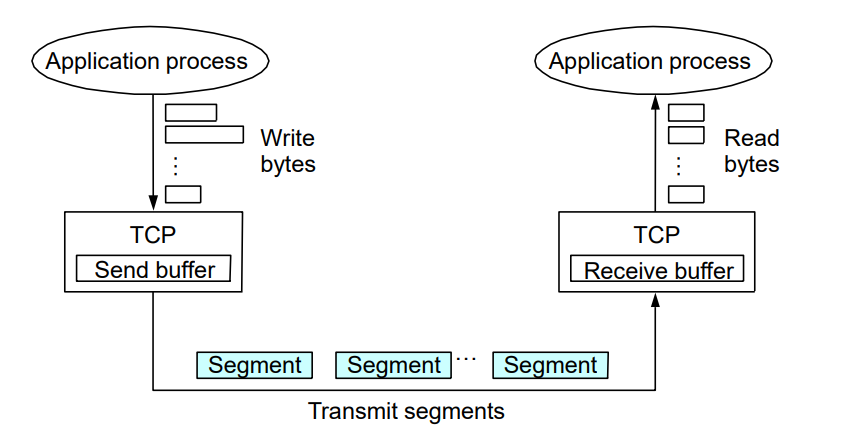
\includegraphics[scale=0.35]{TCPFeatures}
  \label{fig:tcp:features}
  \caption[TCP Features]{A image representing how TCP works}
\end{figure}

\paragraph*{Main features}

TCP has the following characteristics:
\begin{itemize}
\item it's an end-to-end protocol (software only on the end hosts)
\item it establishes a connection\dots
  \begin{itemize}
  \item reliable. A checksum is used to detect bit level errors and sequence
    numbers to detect sequencing errors. This means that, if something arrives
    out of order, TCP reorders it before forwarding it to the application level.
  \item correct
  \item ordered (thanks to sequencing numbers)
  \end{itemize}
\item full duplex
\item it is not so appropriate for current wireless scenarios (but there are
  many variants of TCP)
\item byte-stream oriented. TCP sends segments (packets) through a 
  physical layer (IP, MAC, whatever) and then waits for an ACK. A missing ACK 
  means that the packet was lost.
\item has congestion control: it keeps the sender for overrunning the network
\end{itemize}

TCP does 2 types of control, the \textbf{flow control} in order to avoid
overwhelming the receiver and the \textbf{congestion control} where the flow
slows down when there is a loss of packets.

\section{Reliability in TCP}
Timeouts are used to detect lost packets: this 
requires setting an RTO (\textit{Retransmission Timeout}). If the ACK is lost,
after waiting the RTO, we retransmit that packet. There are obviously some
issues: how much should the RTO be? Are we sure that, in wireless networks,
a missing ACK equals a missing packet?
As for the optimal setting of the RTO, we usually want to wait at least 
one RTT (\textit{Round Trip Time}) before retransmitting. This values have to be
calculated accurately, because a low RTO means unneeded retransmissions, while 
having a high RTO leads to a poor throughput. Basically, the RTO estimator must 
adapt to change in RTT, usually having $RTO=4 \cdot RTT$.

Sequencing numbers are used to detect sequencing errors, meanwhile timeouts
are used to detect lost packets.
RTT determines the speed of TCP connection.

\section{Fast Re-transmission}

\begin{wrapfigure}{r}{0.25\textwidth}
  \begin{center}
    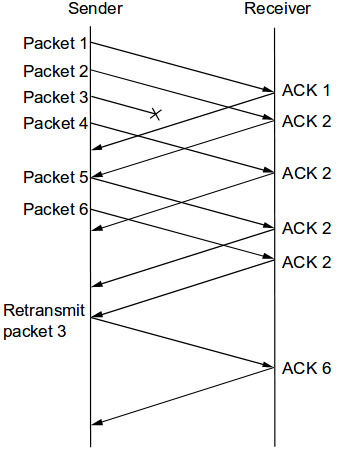
\includegraphics[scale=0.36]{FastRetransmit}
  \end{center}
  \caption[Fast Retransmission example]{}
\end{wrapfigure}

Consider duplicate ACKs, repeated ACKs for the same segment. An ACK is generated
every time we receive a packet, but it doesn't
state the number of the last packet received, instead it returns the number of
the last packet of the longest complete sequence received.
For example: if A sends packets 1-6 without errors, it receives ACK(6). 
Then 7 goes missing and 8 is received. The ACK will be ACK (6). So, we have a 
duplicate ACK (dupack).
Duplicate ACKs occur in case of packet loss, packet re-ordering or 
window update. Generally, we can assume that the receipt of 3 or more dupacks 
indicates a packet loss and so we don't need to wait for the timeout to 
retransmit. This is a faster way to detect packet loss, since the name
\textbf{Fast Retransmit}.
Instead of waiting $4 \cdot RTT$ we resend after $1 \cdot RTT$, which is after
three or ore dupacks.
Duplicate ACKs can happen due to loss of packets, packets re-ordering or flow
control window update.

\section{Fast Recovery}

TCP normally increases the number of 
packets sent by 1 every RTT and, every time a packet is lost, it restarts form
1. In Fast Recovery, instead of going back to 1, we start at SSTHRESH
(\textit{Slow start threshold}), a threshold usually put at about $\frac{1}{2}$
of where we were. Note that even using Fast Recovery we don't have an optimal
situation for wireless networks, having lost a packet due to network errors
doesn't mean I have bandwidth problems and so it doesn't make any sense to slow
down restarting from $\frac{1}{2}$, we should just resend the packet.

\subsection{Congestion Window}
A Congestion Window ($cw$) is used to keep the sender for overrunning the
network sending too many packets. A $cw$ sets the number of packets without ACK
that can be currently traveling in the network. The window starts small and,
every time a whole window has been received (ACKs have been sent back), the
window increases by 1. Otherwise, if some packets are lost, the window either
return to 1 or goes back to the slow start threshold (depending on the TCP
version in use).
\begin{figure}[h]
  \centering
  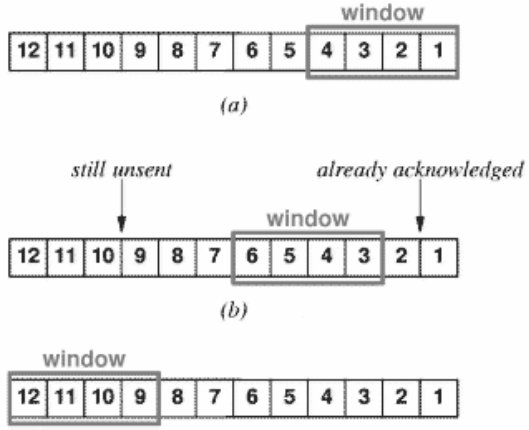
\includegraphics[scale=0.4]{CongestionWindow}
  \caption{Congestion Window schema}
  \label{fig:tcp:cwschema}
\end{figure}

\section{Flow control}

The receiver uses an \textbf{Advertise Window} to manage flow control\footnote{
  As said by the professor during lesson: ``The bandwidth/capacity depends on
  the smallest part of the pipe'' $pipeSize = Delay \cdot Bandwidth$
}. The adWindow is the max number of bytes that it can receive (basically how
much space is left in the buffer). It is communicated back to the sender in the
ACK. 
On the other hand, the sender's actual window is the \textbf{Sending Window} and 
it represents the actual bytes sent out. It corresponds to the minimum between 
its congestion window and the receiver's advertised window
($min(congestion window,\ advertise window)$). 
We can think of the network channel as of a tube and our objective is to 
keep it full at any time (otherwise we would be wasting bandwidth). By
multiplying the bandwidth by the delay ($delay = \frac{RTT}{2}$) we get how much
data we can have in a connection without clogging it. Incidentally, this is also
the max size of the congestion window. When using TCP, to get the size of the
congestion window we calculate $Bandwidth \cdot RTT$, because we also have to
consider ACKs.
\todo{These formulas are not clear enough, please check it out!}

\subsubsection{Additive Increase/Multiplicative Decrease}

The purpose is to adjust changes in the available capacity.
We actually have an additive increase because we increment the $cw$ by one
packet per RTT, which is +1 every time an ACK is received and a Multiplicative
Decrease because, every time a drop is detected via triple-dupacks we set the
$cw=\frac{cw}{2}$. If we plot the cwnd size (or the KB sent) over time we get a
typical saw tooth behavior (Figure~\ref{fig:tcp:sawtooth}). We can see how the
cwnd grows linearly in time and that TCP sends a cwnd's worth of bytes each RTT.

In practice we have:
\begin{itemize}
  \item increment = $\frac{1}{cwnd}$
  \item cwnd += increment
  \item cwnd = $\frac{cwnd}{2}$ if a timeout occurs
\end{itemize}

\begin{figure}[t]
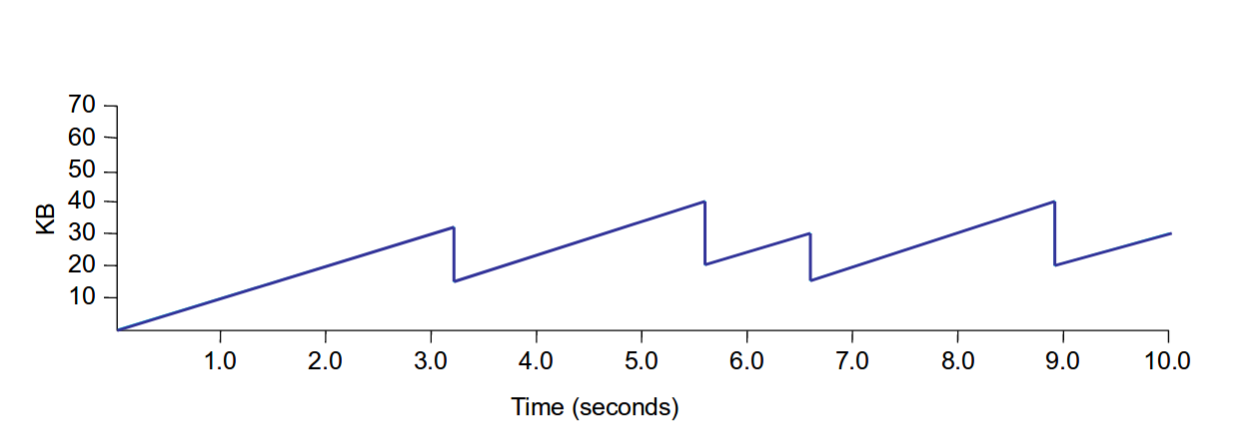
\includegraphics[scale=0.3]{sawtooth.png}
\caption[Saw tooth shape behavior]{Saw tooth shape behavior. Timeouts cause
  \textbf{multiplicative decrease (/2)}}
\label{fig:tcp:sawtooth}
\end{figure}

\subsection{Slow Start Phase SS}

\textbf{Purpose}: quickly determine the available capacity.

\noindent This phase happens before addictive increase. It starts when first
starting connection or when connection goes dead waiting for timeout.

\begin{itemize}
\item begin with cwnd = 1 packet
\item \textbf{double (*2)} cwnd for each RTT (increment by 1 packet for each
  ACK)
\item This is exponential increase to check for available bandwidth (up to half
  of cwnd may get lost)
\end{itemize}

Keep in mind that this phase is not ``slow'', it is exponential.
\textbf{SSTHRESH} (slow start threshold) indicates when to begin additive
increase phase and it's set to one half of $cwnd$ when a packet loss happens.
So, SSTHRESH goes through multiplicative decrease for each packet loss (because
also the $cwnd$ does so).
If we have $cwnd \ge SSTHRESH$ we use congestion avoidance.

SSTHRESH is very large on connection setup.
Since detecting losses with timeout is considered to be an indication 
of severe congestion, when a timeout occurs:	
\begin{itemize}
  \item $SSTHRESH = \frac{cwnd}{2}$ (multiplicative decrease)
  \item $cwnd=1$
  \item $RTO=RTO \cdot 2$
  \item Enter slow start
\end{itemize}

Note that $cwnd$ and SSTHRESH always $\ge$ 1 MSS\footnote{
MSS stands for \textit{Maximum Segment Size}, and it's a parameter of the
options field of the TCP header that specifies the largest amount of data,
specified in bytes, that a computer or communications device can receive in a
single TCP segment.
}. 

\begin{figure}[t]
  \centering
  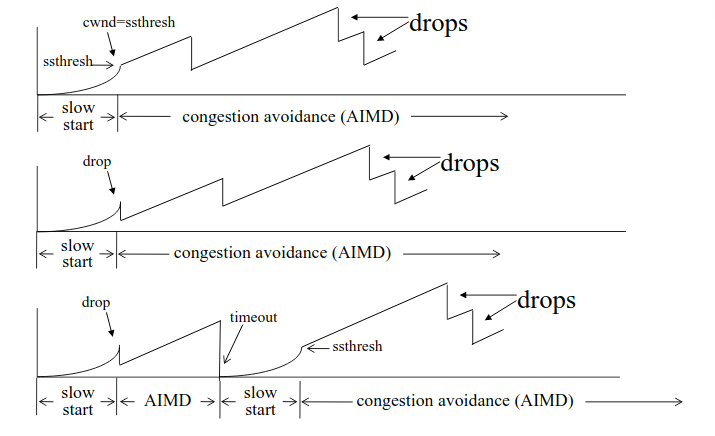
\includegraphics[scale=0.5]{TCPBeh}
  \caption{TCP behavior using AIMD and Slow Start}			
  \label{fig:tcp:TCPBeh}
\end{figure}

\subsubsection{Summary}	
	Summarizing, the complete congestion control functionality works in 2 
phases:
\begin{itemize}
  \item \textbf{Slow Start Phase}: until $cwns \le SSTHRESH$.
Exponential growth, at each returning ACK a new packet is transmitted 
($cwnd=cwnd+1$) and at every RTT $cwnd=cwnd \cdot 2$; 
  \item \textbf{Congestion Avoidance}: when $cwnd > SSTHRESH$. We 
switch to linear growth, at each returning ACK a new packet is transmitted 
($cwnd=\frac{cwnd+1}{cwnd}$) and at every RTT $cwnd=cwnd+1$.
\end{itemize}
	
We have two ways to detect losses: 
\begin{itemize}
  \item \textbf{Timeouts}: we set $SSTHRESH=\frac{cwnd}{2}$ and $cwnd=1$
(or, restart in Slow Start Phase);
  \item \textbf{Three Dupacks}: $SSTHRESH=\frac{cwnd}{2}$, $cwnd=\frac{cwnd}{2}$
(and restart from congestion avoidance phase).		 
\end{itemize}
	
Finally, see Figure~\ref{fig:tcp:TCPCC} and~\ref{fig:tcp:TCPSawSum} for details.
	
\begin{figure}[t]
  \centering
  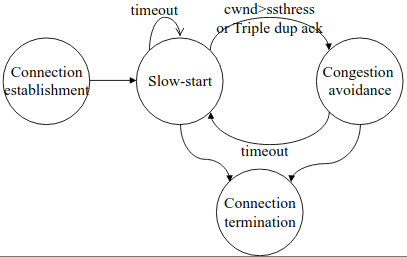
\includegraphics[scale=0.5]{TCPCC}
  \caption{TCP Congestion Control Summary}
  \label{fig:tcp:TCPCC}
\end{figure}

\begin{figure}[t]
  \centering
  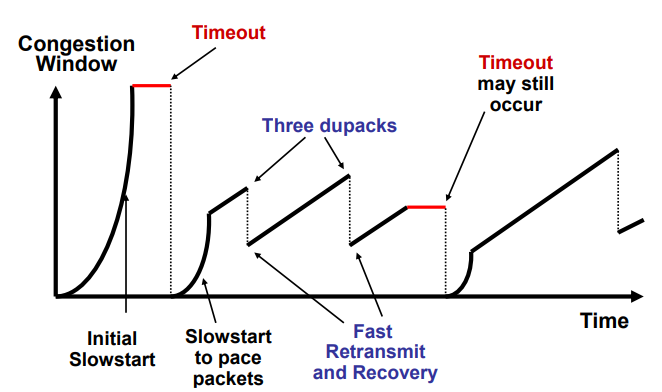
\includegraphics[scale=0.4]{TCPSawSum}
  \caption{TCP Saw Tooth Explained}
  \label{fig:tcp:TCPSawSum}
\end{figure}

\subsection{Loss recovery}
There are two ways to detect losses: time outs and three dupacks.
With timeout expiration:
\begin{itemize}
  \item $ssthresh = \frac{cwnd}{2}$
  \item $cwnd = 1$ (so, restart in SS phase)
\end{itemize}
With three dupacks:
\begin{itemize}
  \item $ssthresh = \frac{cwnd}{2}$
  \item $cwnd = \frac{cwnd}{2}$ (so, restart in cong. avoidance phase)
\end{itemize}
